\begin{figure}[htp]
\centering
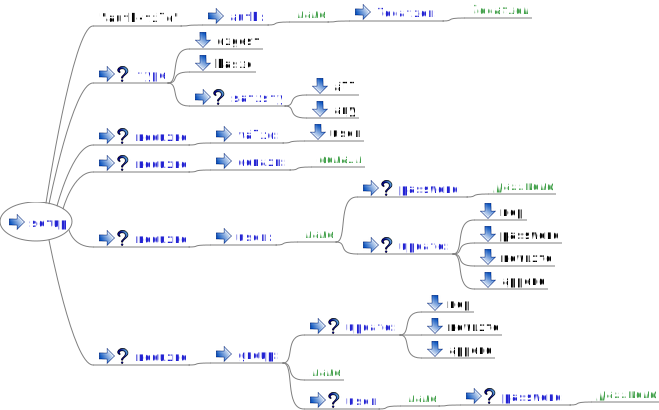
\includegraphics[width=0.99\textwidth]{httpd_setup_auth_file_script}
\label{fig:httpd_setup_auth_file_script}
\caption{Httpd File Authentication Statements}
\end{figure}

%% setup auth-file
\TheStatement[httpd:domain:setup-auth-file]{setup ``auth-file''}
\TheStatement*[httpd!domain!setup!auth-file]{setup ``auth-file'', auth: \Arg{name}, location: \Arg{location}, \{ type require \}}

Configures authentication with a file as the storage for groups and users,
with the \Arg{name} of the authentication and the \Arg{location} that is 
restricted.

\begin{lstlisting}[style=Java]
httpd {
    domain "test1.com", address: "192.168.0.50", {
        setup "auth-file", auth: "Private Directory", location: "/private", {
        }
    }
}
\end{lstlisting}

%% type
\TheStatement[httpd:domain:setup-auth-file-type]{type}
\TheStatement*[httpd!domain!setup!auth-file!type]{type \Type{digest|basic} [, satisfy: \Type{all}| \Type{any}]}

The \qcode{type} statement sets the authentication types. The 
authentication can be 
\begin{asparaitem}
\item \qcode{digest} MD5 digest authentication;
\item \qcode{basic} HTTP basic authentication;
\end{asparaitem}

The \qcode{satisfy} statement sets the criteria that must be satisfied to 
allow access to a resource.
\begin{asparaitem}
\item \qcode{all} all criteria must be met;
\item \qcode{any} only one criteria must be met;
\end{asparaitem}

\begin{lstlisting}[style=Java]
httpd {
    domain "test1.com", address: "192.168.0.50", {
        setup "auth-file", auth: "Private Directory", location: "/private", {
            type AuthType.digest, satisfy: SatisfyType.any
        }
    }
}
\end{lstlisting}

%% require valid
\TheStatement[httpd:domain:setup-auth-file-require-valid]{require valid}
\TheStatement*[httpd!domain!setup!auth-file!require valid]{require valid: \Type{user}}

Sets the required valid mode. The mode can be 
\begin{asparaitem}
\item \qcode{user} require valid user;
\end{asparaitem}

\begin{lstlisting}[style=Java]
httpd {
    domain "test1.com", address: "192.168.0.50", {
        setup "auth-file", auth: "Private Directory", location: "/private", {
            require valid: RequireValid.user
        }
    }
}
\end{lstlisting}

%% require domain
\TheStatement[httpd:domain:setup-auth-file-require-domain]{require domain}
\TheStatement*[httpd!domain!setup!auth-file!require domain]{require domain: \Arg{domain}}

Sets the required \Arg{domain}.

\begin{lstlisting}[style=Java]
httpd {
    domain "test1.com", address: "192.168.0.50", {
        setup "auth-file", auth: "Private Directory", location: "/private", {
            require domain: "https://%"
        }
    }
}
\end{lstlisting}

%% require user
\TheStatement[httpd:domain:setup-auth-file-require-user]{require user}
\TheStatement*[httpd!domain!setup!auth-file!require user]{require user: \Arg{name} [, password: \Arg{password}] [, update: \Type{nop}| \Type{password}| \Type{rewrite}| \Type{append}]}

Adds the required user with the set \Arg{name} and with the optional \Arg{password}.
If the user was already set in the authentication database, the script can
update the password of the user with the \code{RequireUpdate\#password}
option, \code{RequireUpdate\#rewrite} rewrites the authentication database,
\code{RequireUpdate\#append} appends the user to the database or
\code{RequireUpdate\#nop} do nothing.

\begin{lstlisting}[style=Java]
httpd {
    user "test1.com", address: "192.168.0.50", {
        setup "auth-file", auth: "Private Directory", location: "/private", {
            require user: "foo", password: "foopassword"
            require user: "bar", password: "barpassword", update: RequireUpdate.password
        }
    }
}
\end{lstlisting}

%% require group
\TheStatement[httpd:domain:setup-auth-file-require-group]{require group}
\TheStatement*[httpd!domain!setup!auth-file!require group]{require group: \Arg{name} [, update: \Type{nop} | \Type{rewrite} | \Type{append}], \{ user \}}

Adds the required group with the set \Arg{name} and with the optional users.
If the group was already set in the authentication database, 
\code{RequireUpdate\#rewrite} rewrites the authentication database,
\code{RequireUpdate\#append} appends the group to the database or
\code{RequireUpdate\#nop} do nothing.

\begin{lstlisting}[style=Java]
httpd {
    group "test1.com", address: "192.168.0.50", {
        setup "auth-file", auth: "Private Directory", location: "/private", {
            require group: "admin1", {
                user "adminfoo1", password: "adminfoopassword"
                user "adminbar1", password: "adminbarpassword"
            }
            require group: "foo1", update: RequireUpdate.append, {
                user "foo1", password: "foopassword"
                user "bar1", password: "barpassword"
            }
        }
    }
}
\end{lstlisting}
